% Figs. 3 and 4 belong to Section III-A; background.tex inputs this file at its end,
% so the two figures pair at the top of the page where Section III starts
\begin{figure}[t]
\centering
\begin{tikzpicture}[>=stealth, font=\scriptsize,
  slot/.style={draw, minimum width=2.3cm, minimum height=0.42cm, inner sep=0pt},
  outv/.style={draw, minimum width=1.0cm, minimum height=0.42cm, inner sep=0pt,
    font=\ttfamily\scriptsize},
  hid/.style={outv, fill=white}, ran/.style={outv, fill=black!10},
  val/.style={outv, fill=black!28}]
% six slots and their outputs, on a common grid
% the outputs are shaded by what the attacker learns of each slot
\foreach \n/\l/\o/\s [count=\k from 0] in
  {t/timer handler/None/val, d/disk handler/None/hid, z/NOP handler/None/hid,
   s/scheduler/None/val, v/private user/None/ran, u/public user/Some o/val}
  {\node[slot] (\n) at (3.0, 1.05-0.42*\k) {\l};
   \node[\s] (o\n) at (5.15, 1.05-0.42*\k) {\o};
   \draw[->] (\n.east) -- (o\n.west);}
\node[draw, dashed, rounded corners=2pt, fit=(t)(u), inner sep=3pt] (pool) {};
\node[draw, rounded corners=2pt, fit=(ot)(ou), inner sep=2pt] (tuple) {};
\node[anchor=south] at (pool.north) {pool: six slots in \texttt{par}};
% the output is a product, the input a sum: the operator is in the title
\node[anchor=south] at (tuple.north |- pool.north) {output: $\times$};
% global state, vertically centred on the pool
\node[draw, rounded corners=2pt, minimum width=1.3cm, minimum height=1.1cm,
  align=center] (sta) at (0.35, 0 |- pool.center) {global\\state\\[1pt]{\tiny (Fig.~\ref{fig:state})}};
% the input is a sum, laid out like the output: disk (inl) white, timer (inr) dark
\node[hid, minimum width=0.85cm, font=\scriptsize] (id) at ($(-1.4, 0 |- sta.center)+(0,0.21)$) {disk};
\node[val, minimum width=0.85cm, font=\scriptsize] (it) at ($(-1.4, 0 |- sta.center)+(0,-0.21)$) {timer};
\node[draw, rounded corners=2pt, fit=(id)(it), inner sep=2pt] (input) {};
\node[anchor=south] at (input.north) {input: $+$};
\draw[->] (input.east) -- (sta.west);
\draw[->] (sta.east) -- node[above] {pid} (pool.west |- sta.east);
\draw[->] (tuple.east) -- ++(0.5,0) node[right] {out};
\draw[->] ($(tuple.east)+(0.25,0)$) |- ($(pool.south)+(0,-0.35)$) -|
  node[pos=0.25, below] {fed back (\texttt{loop})} (sta.south);
% key: the shades as nested sets
\begin{scope}[shift={(-1.2,-2.25)}]
\draw[rounded corners=3pt, fill=white] (0,0) rectangle (7.6,-0.62);
\draw[rounded corners=3pt, fill=black!10] (2.25,-0.08) rectangle (7.5,-0.54);
\draw[rounded corners=3pt, fill=black!28] (5.1,-0.15) rectangle (7.4,-0.47);
\node[anchor=west] at (0.05,-0.31) {tells nothing apart};
\node[anchor=west] at (2.3,-0.31) {tells \texttt{Some} from \texttt{None}};
\node[anchor=west] at (5.15,-0.31) {\dots\ and every value};
\end{scope}
\end{tikzpicture}
\caption{The model. An interrupt only updates the global state. The state's pid
  selects one slot, which takes a step and emits \texttt{Some o}; every other slot
  emits \texttt{None}. Because the slots are composed with \texttt{par}, their
  outputs form a product, a six-tuple, which is emitted and fed back to update the
  state. The input is a sum of the two interrupts. Each position of the output, and
  each alternative of the input, is shaded by which of its values the attacker can
  tell apart (key below).}
\label{fig:system}
\end{figure}
\begin{figure}[t]
\centering
% the global state of fig:system, field by field (models.v, state_type);
% shading: public (dark) or private (white) to the attacker under the state
% equivalence of sec:state-equiv
% laid out like the columns of fig:system: a framed column with its operator in the
% title, a nested sum or product side by side within a row
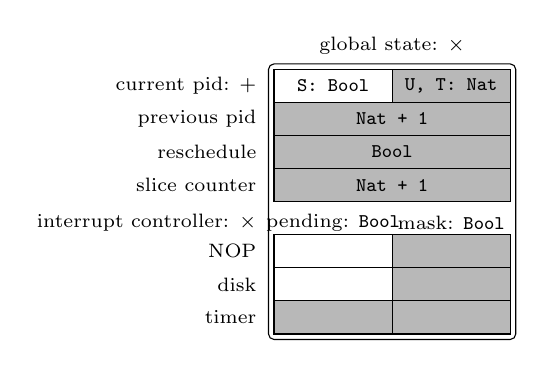
\begin{tikzpicture}[font=\scriptsize,
  c/.style={draw, minimum height=0.42cm, inner sep=0pt, font=\ttfamily\scriptsize},
  pub/.style={c, fill=black!28}, priv/.style={c, fill=white}]
% fields, one row each, cells spanning x = 0 .. 3.0
\node[anchor=east] at (-0.1,0) {current pid: $+$};
\node[priv, minimum width=1.5cm] at (0.75,0) {S: Bool};
\node[pub, minimum width=1.5cm] at (2.25,0) {U, T: Nat};
\foreach \y/\l/\t in {-0.42/previous pid/Nat + 1, -0.84/reschedule/Bool,
                      -1.26/slice counter/Nat + 1}
  {\node[anchor=east] at (-0.1,\y) {\l};
   \node[pub, minimum width=3.0cm] at (1.5,\y) {\t};}
% the interrupt controller: one entry per handler, each pending x mask
\node[anchor=east] at (-0.1,-1.74) {interrupt controller: $\times$};
\node at (0.75,-1.74) {pending: \texttt{Bool}};
\node at (2.25,-1.74) {mask: \texttt{Bool}};
\foreach \y/\l/\p in {-2.1/NOP/priv, -2.52/disk/priv, -2.94/timer/pub}
  {\node[anchor=east] at (-0.1,\y) {\l};
   \node[\p, minimum width=1.5cm] at (0.75,\y) {};
   \node[pub, minimum width=1.5cm] at (2.25,\y) {};}
\draw[rounded corners=2pt] (-0.07,-3.22) rectangle (3.07,0.28);
\node[anchor=south] at (1.5,0.28) {global state: $\times$};
\end{tikzpicture}
\caption{The global state of \cref{fig:system}, field by field, laid out and shaded
  as there (\cref{sec:state-equiv}). The current pid is a sum: its \texttt{inl}
  side holds a secret handler (an S step), a \texttt{Bool} saying which one, and
  its \texttt{inr} side the number of any other process (U or T). Its
  equivalence is $\privvis + \pubeq$ (\cref{def:visible}), so
  the tag is public: whether a secret handler runs is public; which one runs is private.
  So are the pending bits of the NOP and disk handlers. Every other field,
  \texttt{None} included, is public.}
\label{fig:state}
\end{figure}
